\subsection{Description du sujet de stage}
\subsubsection{L'environnement de simulation: SE-STAR}

SE-STAR est un logiciel de simulation dans des environnements modélisés à partir
de lieux réels. Dans l’environnement virtuel interagissent en temps réel des
agents représentant des personnes. Il est conçu en particulier pour les
infrastructures critiques (stations de métro, gares, aéroports).
Il peut gérer en temps réel un grand nombre d’agents (plus de 10 000), permettant de nombreuses interactions avec l’environnement qui peut être facilement modifié par l’utilisateur (ajout d’objets tels que des caméras de surveillance, des distributeurs de boissons, des bancs, etc.). La simulation cherche à représenter de manière réaliste le comportement des usagers de ces infrastructures. 

Dans le contexte de ce stage, nous allons restreindre SE-STAR à la modélisation d'un environnement simple contenant un seul agent. 

\midskip
\begin{figure}[!h]
\centering
\begin{subfigure}{.5\textwidth}
  \centering
  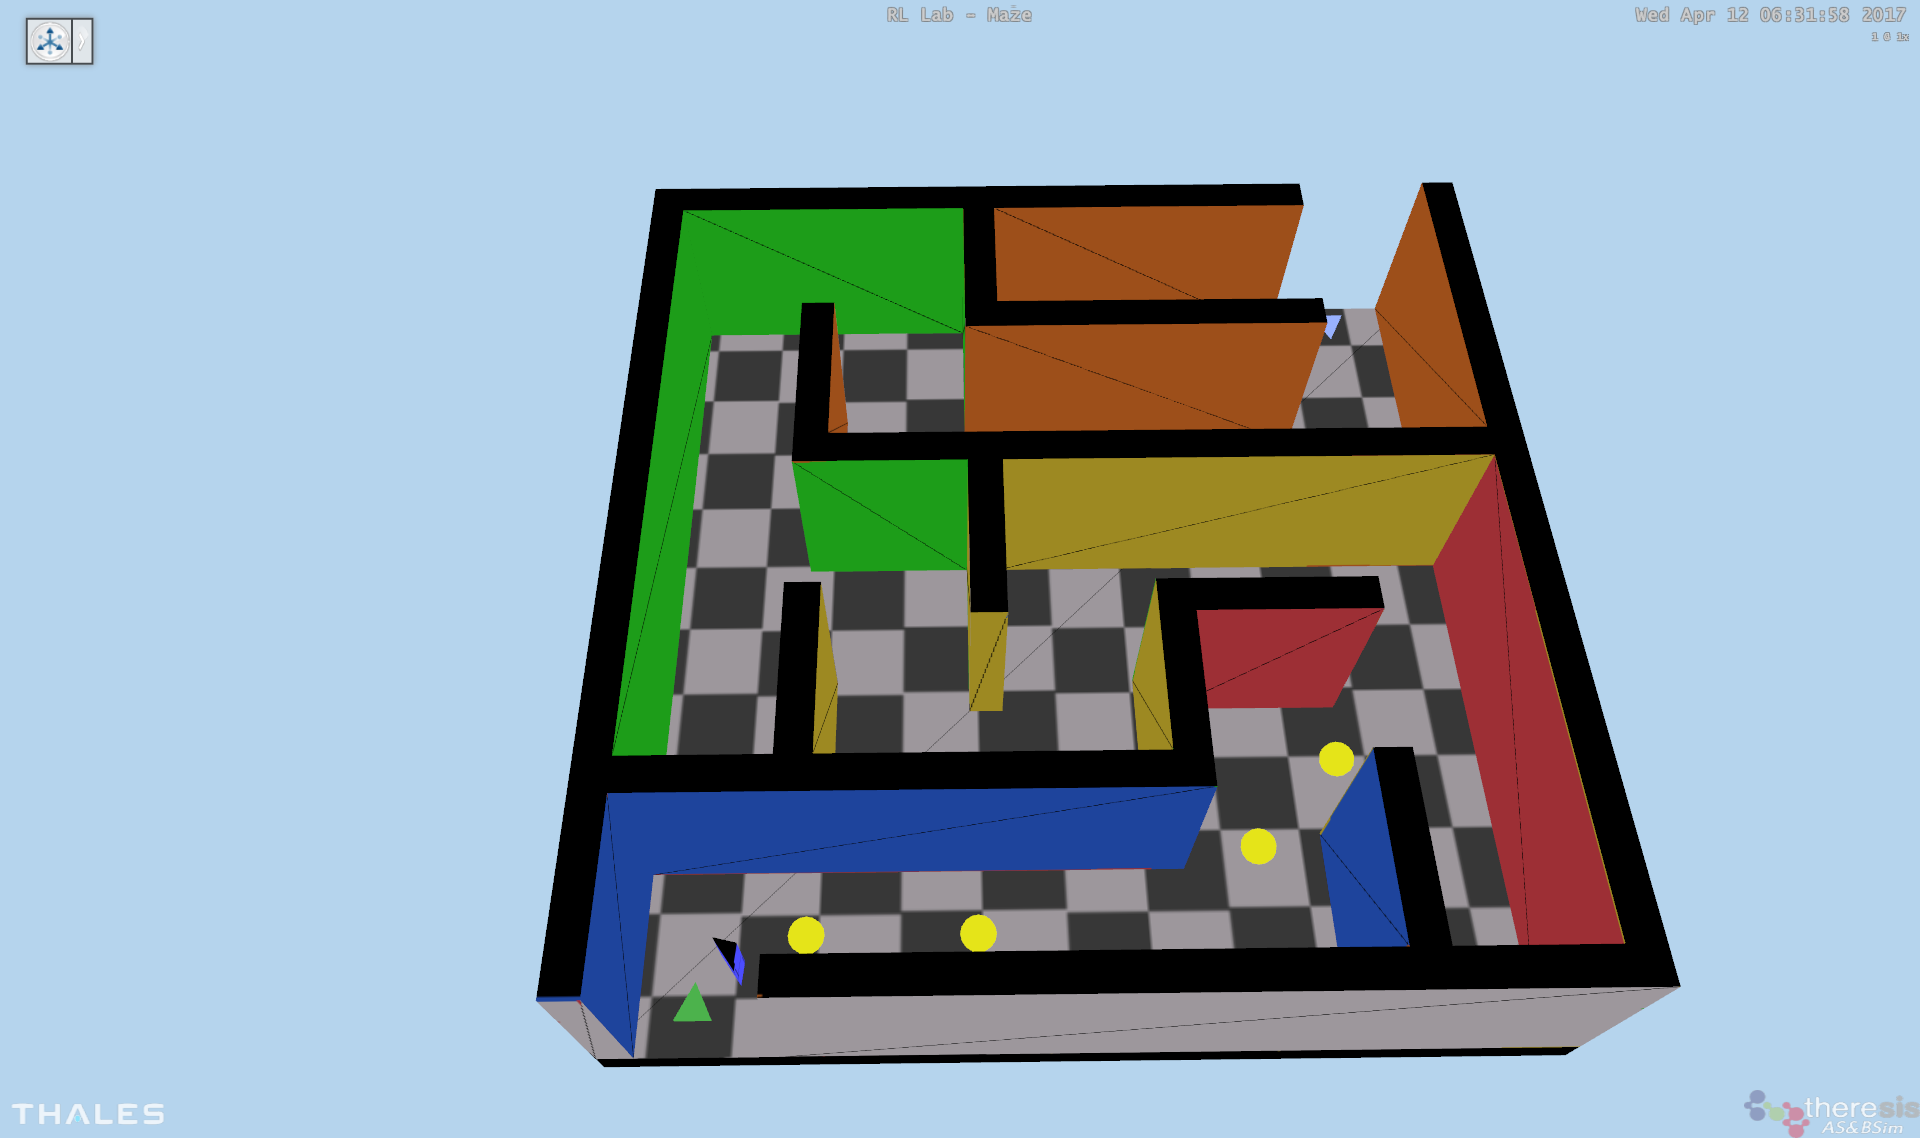
\includegraphics[width=.9\linewidth]{./assets/SESTAR/env_sestar_color.png}
  \caption{Environnement créé pour le contrôle d'un agent}
  \label{fig:sub1}
\end{subfigure}%
\begin{subfigure}{.5\textwidth}
  \centering
  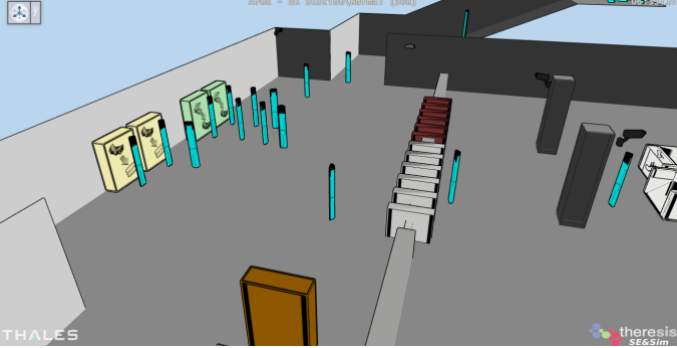
\includegraphics[width=.9\linewidth]{./assets/SESTAR/sestar_metro.png}
  \caption{Simulation d'une station de métro}
  \label{fig:sub2}
\end{subfigure}
\caption{Exemple d'utilisation de SE-STAR}
\label{fig:test}
\end{figure}

\subsubsection{Objectif du stage et contraintes identifiées}


L'objectif de ce stage est de proposer un contrôle d'un agent de l'entrée de l'environnement à la sortie de l'environnement en évitant des zones considérées comme dangereuses. Néanmoins, nous possédons des contraintes sur notre contrôle:     

\begin{enumerate}
    \item \textbf{L'environnement est inconnu de l'agent:}
    \smallskip
    
    La première contrainte de notre objectif est que notre environnement est inconnu. En effet nous souhaitons développer un algorithme de contrôle que soit capable de proposer un asservissement fiable pour tout environnement proposé par SE-STAR. L'impératif de généralisation est une contrainte forte pesant sur le choix technologique pour réaliser ce contrôle. En effet, un asservissement classique repose sur la connaissance de la dynamique du système qui n'est pas disponible dans notre cas et , pire encore, est fluctuante en fonction des environnements.
    
    \item \textbf{Le contrôle doit être robuste aux changements d'environnements:}
    \smallskip
    
    Pour être utile, il faut que notre agent apprenne à se mouvoir d'un point A à un point B. De plus, notre algorithme d'apprentissage ne doit pas se suffire à apprendre par coeur la séquence d'action pour rejoindre la sortie mais doit apprendre à se repérer et voir les points d'intérêts permettant de trouver la sortie quelque soit l'environnement. Nous recherchons une approche analogue à la façon humaine  pour sortir d'un environnement (longer les murs, chercher des indices visuels indiquant la sortie ...).
 
    \item \textbf{Les entrées de la commande sont données par la vision de l'agent:}
    \smallskip
    
    Une des difficultés qui empêche l'utilisation des outils de la théorie du contrôle, vient du format des entrées. Nous devons bâtir un algorithme de contrôle se basant sur des images partielles d'un environnement. Comme un humain lâché dans un labyrinthe, il n'aura pas accès à une image complète du labyrinthe mais uniquement une vue partielle possiblement bruitée. Notre agent devra, à partir d'une information incomplète, réussir à déterminer une séquence d'actions lui permettant de trouver la sortie.
    
  
\end{enumerate}

\subsubsection{Défis et choix technologiques}

Nous cherchons un algorithme de contrôle assez générique pour ne nécessiter en entrée que des images (tableaux de pixels). Un des défi de ce stage est de permettre à  l'agent d'être capable de trouver les repères les plus adaptés pour réussir sa mission quelque soit l'environnement.

Cela implique que nous ne recherchons pas seulement une solution adaptée à un environnement particulier. Nous souhaitons un agent capable de généraliser à un ensemble d'environnements similaires la recherche d'une politique quasi optimale. 

Les nombreuses contraintes et les défis technologiques impliquent une décomposition de l'algorithme choisi en deux grandes étapes:

\begin{enumerate}
    \item L'agent explore l'environnement et apprend simultanément une politique optimale pour arriver à la sortie.
        % coeur -> e dans le o
    \item Nous nous assurons que l'agent est capable de trouver une bonne politique sur des environnements similaires pour vérifier que l'agent n'a pas juste \emph{appris par coeur une solution}.
\end{enumerate}

Se pose naturellement la question du choix de la technologie pour réaliser cet apprentissage.
La contrainte de généralisation nous pousse à utiliser l'apprentissage profond (ou \emph{deep learning}). L'apprentissage profond a prouvé son efficacité dans sa capacité à être pertinent à un grand nombre d'entrées possibles.  
La distinction entre généralisation et apprentissage par coeur des données est particulièrement importante dans ce domaine. Les méthodes qui en sont issues ont prouvé leurs capacité à trouver des solutions à des problèmes nouveaux (jamais utilisés en entrainement).

Il nous faut un domaine s'attaquant à des environnements compliqués, observés de manières partielles, et possiblement changeant au cours du temps. L'apprentissage par renforcement propose une manière d'aborder ce genre d'environnement complexe. 

Ainsi, nous avons proposé une méthode alliant l'apprentissage profond pour gérer les entrées du système avec l'apprentissage par renforcement pour réaliser un agent capable de naviguer dans un environnement pour y découvrir une sortie en ayant comme donnée unique sa vision.
